\section{Introduction}\label{introduction}

Technological advances have transformed how museums document, present and interpret their collections. Immersive experiences are realised through tools such as 3D printing and virtual reality \cite{allard2005use,Wachowiak01082009,RCM_2024_3D,Kuzminsky_LaserScan_2012,Schaich_3D_2007}. These technologies form a kind of experiential authenticity, enabling encounters that evoke the past's sensory, emotional, and intellectual essence \cite{trant_Auth_1999}. However, as Pine and Gilmore note \cite{pinegilmore_2007}, achieving authenticity requires museums to navigate the delicate balance between preservation and meaningful engagement—a challenge that is particularly evident in the case of historical musical instrument collections \cite{McAlpine2014}.

Musical instruments represent a peculiar fusion of form, function, and history. Their cultural value extends beyond their visual appeal to include the tactile and auditory dimensions of use \cite{Fritz2017}. Yet, preservation concerns often limit direct interaction, reducing these artefacts to static displays. This ``red velvet cord'' approach, as theorised by McAlpine \cite{McAlpine2014}, protects fragile mechanisms but diminishes the instruments’ functional identity, disconnecting visitors from the full richness of their historical and cultural context.

The \anon{Tagliavini} Collection in \anon{Bologna \cite{Tagliavini2007}}, renowned for its historical keyboard instruments, exemplifies this dilemma. Housed at Museo San Colombano - Genus Bononiae, with more than seventy early keyboard instruments, primarily early plucked stringed keyboards of italian origin. The collection stands out as a valuable resource for musicologists, organologists and musicians alike. Preserving the instruments' authenticity was the cornerstone of \anon{Ferdinando Tagliavini}’s vision. This guiding principle led him to collect instruments which could be restored to playing condition after minimal intervention. 

However, the delicate mechanisms of these instruments and their historical significance mean they are only played under strict conditions—by experienced historical keyboard performers or by young musicians under strict supervision from the curator. 
To enhance accessibility and engagement, the museum commissioned the replica (Figure \ref{fig:teaser}) of a historical keyboard built in the tradition of the Italian school, which is the subject of this paper.
The keyboard, which museum visitors can use without special permission, presents two choirs of muted strings and can generate MIDI messages. The interface is currently connected to a commercial software sampler, though the ultimate goal is to render accessible the sound of instruments that can not be kept on a playing condition. Museum visitors are invited to play the interface and listen through a pair of headphones. This work outlines the technological aspects of the interface's construction and offers reflections on its role within the \anon{Tagliavini} Collection and potential application within the wider musical instrument museum context. 

As part of the initiative to improve the accessibility of museums, the Museo San Colombano - Tagliavini Collection, part of the cultural itinerary of Fondazione Carisbo, has designed a series of projects to improve cognitive and sensory accessibility at different levels, in a project funded by NextGenerationEU. The aim of this project is to exploit the potential of the collection of musical instruments to create an immersive experience and interaction with the heritage on display. 
reinterpretation of the historical musical objects in their tactile-auditory dimension aims to open up the exhibition to blind and partially sighted visitors. The augmented keyboard fulfils many of the project's aims and is part of the initiative to allow visitors of different abilities to engage in a hands-on creative process within the museum.

\section{Related Work and Motivations}\label{related-work}

Museums face a constant tension between accessibility and preservation, restricting how visitors can interact with collections \cite{Templeton2018, McAlpine2014}. For musical instrument museums, these challenges are compounded by the difficulty of preserving historical instruments in a playable condition \cite{McAlpine2014}. The instruments' inherent fragility and gradual decay inevitably result in a point where they can no longer be played, even when collections adhere to the strictest conservation protocols \cite{NYT_strad}. A marked cultural change has taken place in recent decades, shifting the focus from the playability of the originals to their conservation. Karp \cite{Karp1979,Karp1985} advocates for a deeper understanding of musical instruments so that enough knowledge is generated to make them as ``copyable'' as possible.

McAlpine discusses a case similar to the \anon{Tagliavini} collection in his examination of the Benton Fletcher Collection at National Trust Fenton House \cite{McAlpine2014}. When these instruments were donated, Benton Fletcher stipulated that they remain playable and should continue to be maintained for tuition and public performance. A large sampling campaign was conducted, and a custom MIDI interface was designed to fulfil this requirement while preserving the original instruments' integrity. The MIDI controller, comprising two commercially available keyboards mimicking the two-manual harpsichord layout, was used by visitors to trigger the instrument samples recorded with tailored strategies for each. However, user tests identified a limitation: the commercially available weighted keys failed to provide an authentic sense of interacting with a historical plucked keyboard instrument \cite{McAlpine2014}. 

On the other hand, the ``Tromba Moderna'' project \cite{Baldwin2016}, a previous NIME initiative, approached the issue of musical heritage playability by recreating and augmenting a replica of a historical tromba marina. A piezo transducer was connected to a sound synthesis engine and a driver within the instrument to simulate the expected vibrations of a historical tromba marina. 


The keyboard presented here inherits some aspects from the Tromba Moderna project. The project aims to offer a tool to enhance the fruition of the \anon{Tagliavini} collection while retaining a form of continuity with historical instrument-building traditions. However, the electronics hidden inside the interface are not intended to augment or disrupt the tactile feedback; rather, they serve as the silent and invisible link between the mechanical and the digital realms. 
The optical sensing technique for the keyboard is adapted from a similar project on the piano by McPherson \cite{McPherson2013}. 
Thus, whether the interface proposed here is a \emph{new} musical interface is subject to discussion, particularly regarding the keyboard's tactile response designed to adhere to longstanding harpsichord building traditions. This work complements and follows up on previous reflections within the NIME community, emphasising the \emph{O} in NIME -- the methodologies and reasoning for exploring `old' instrument designs at NIME \cite{Masu_NIME_2023}. 
\textcolor{red}{ALT: This work has incorporated and developed further the ideas of reusing and complimenting the `old' in digital musical instrument design as put forward in `The \emph{O} in NIME' \cite{Masu_NIME_2023}}.
The intended use of the keyboard through meaningful interaction with a museum exhibit is where the novelty of this work lies, rather than solely in its technological development. Relying on previous NIMEs, this project extends the longevity of the results beyond the scope envisaged in the original works, enhancing their sustainability, as discussed by Masu \emph{et al.} \cite{Masu_NIME_2023}.

Besides enhancing the visitor experience, future design iterations will serve as a research tool to explore the unique characteristics of the harpsichord and its impact on performance through the \anon{ERC-funded NEMUS} project \anon{\cite{NEMUS}}, aiming to virtually reproduce the sound of antique keyboard instruments, and upcoming projects such as Rem@ke \cite{remake1} investigating embodied relationships between instrument and performer.

\begin{figure*}
\centering
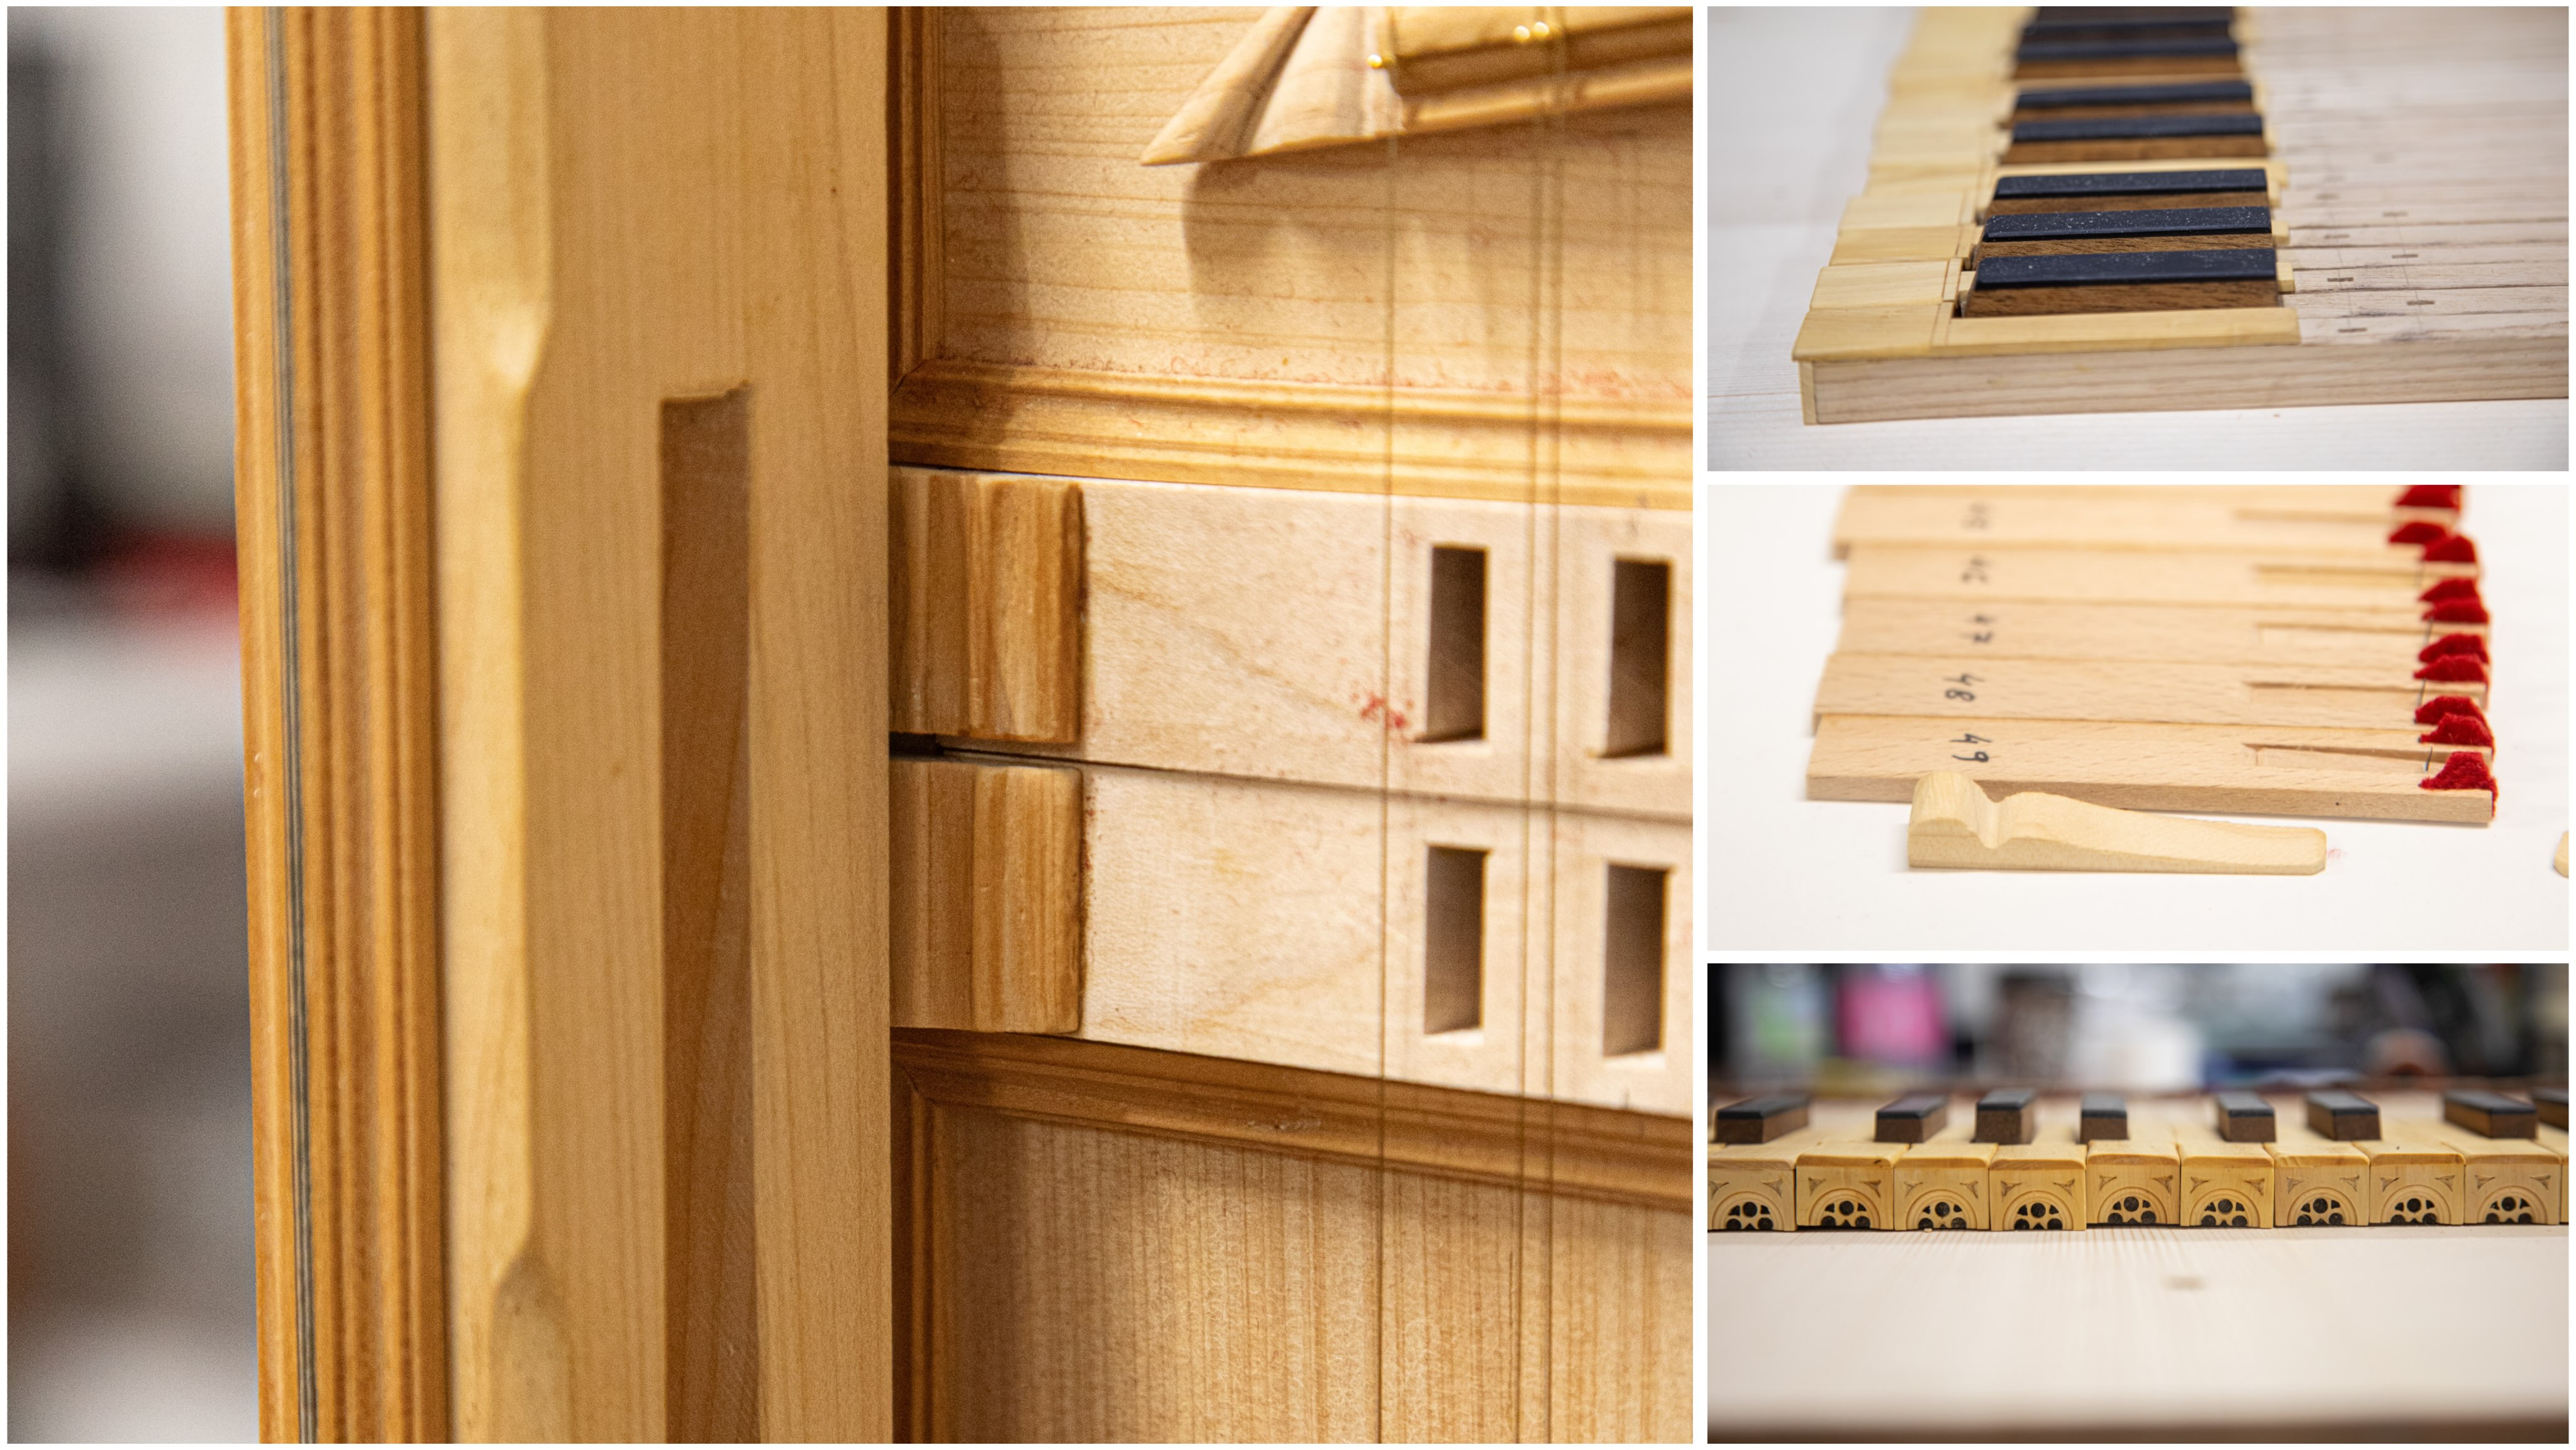
\includegraphics[width=0.8\linewidth]{src/images/details.jpg}
\caption{Details of the replica, including the key slots and sides, keys, and jacks with seagull plectra.}
\label{fig:details}
\end{figure*}

\section{Design Principles}\label{design}

The design of the augmented replica keyboard for the \anon{Museo San Colombano - Genus Bononiae} was guided by three principal constraints stipulated by the museum:

\begin{itemize}
    \item \emph{Faithfulness}. The keyboard mechanism ensured fidelity to its authentic operation. The electronics system would not seek to `fix' or `improved' on limitations of the original design.     
    \item \emph{Robustness and reliability}. The system needed to accommodate frequent use by museum visitors and allow for straightforward maintenance by staff without requiring specialised technical expertise.
    \item \emph{No visible electronics}. To preserve the visual integrity of the exhibit, all electronic components had to remain concealed except for a pair of headphones and a small display for audio parameter adjustments.
    \item \emph{Reduced use of space}. As museums often face space limitations, the instrument needed be compact enough not to compromise space for exhibition of the permanent display. 
\end{itemize}

These constraints demanded an electronics system that was non-invasive in design and that was respectful of the historical aesthetics of the instruments. The requirement for faithfulness to the original mechanism immediately ruled out a mechanical design reliant on electromechanical actuators, as in previous works on piano haptics \cite{Timmermans2020,Gillespie1996}. 
While actuators can generate considerable force, it is difficult to achieve a jack's free motion and resistance without extensive mechanical intervention such as that carried out by Gillespie \cite{Gillespie1996}. A recreation of the mechanism can already achieve the tactile realism of the harpsichord.
It should first be determined if mechanical recreation is sufficient as part of a digital musical instrument before pursuing elaborate electromechanical emulation. 

The final design, shown in Figures \ref{fig:teaser} and \ref{fig:details}, is a 49-key, two-register harpsichord keyboard replica. The keyboard layout was deliberately modelled after early Italian harpsichords, leveraging the human tendency to be influenced by visual elements when making musical judgments \cite{Tsay2013}. This effect is particularly relevant in musical instruments, as demonstrated by studies conducted by Fritz \emph{et al.} \cite{Fritz2012, Fritz2014, Fritz2017}. Instead of attempting to mitigate this influence, the design embraces it. This phenomenon, akin to a `musical instrument McGurk effect’, is one of the reasons why the electronics have been concealed from view. The aesthetics of the interface enhance its likelihood of being perceived as an `authentic' musical instrument. Given the extensive research into modelling and recreating piano action \cite{Cadoz1990, Gillespie1996, Timmermans2020}, the visual component may provide the final persuasive element necessary for acceptance, similar to the way visual perception affects judgments of musical performance \cite{Tsay2013}.

\begin{figure}[!b]  
  \centering
  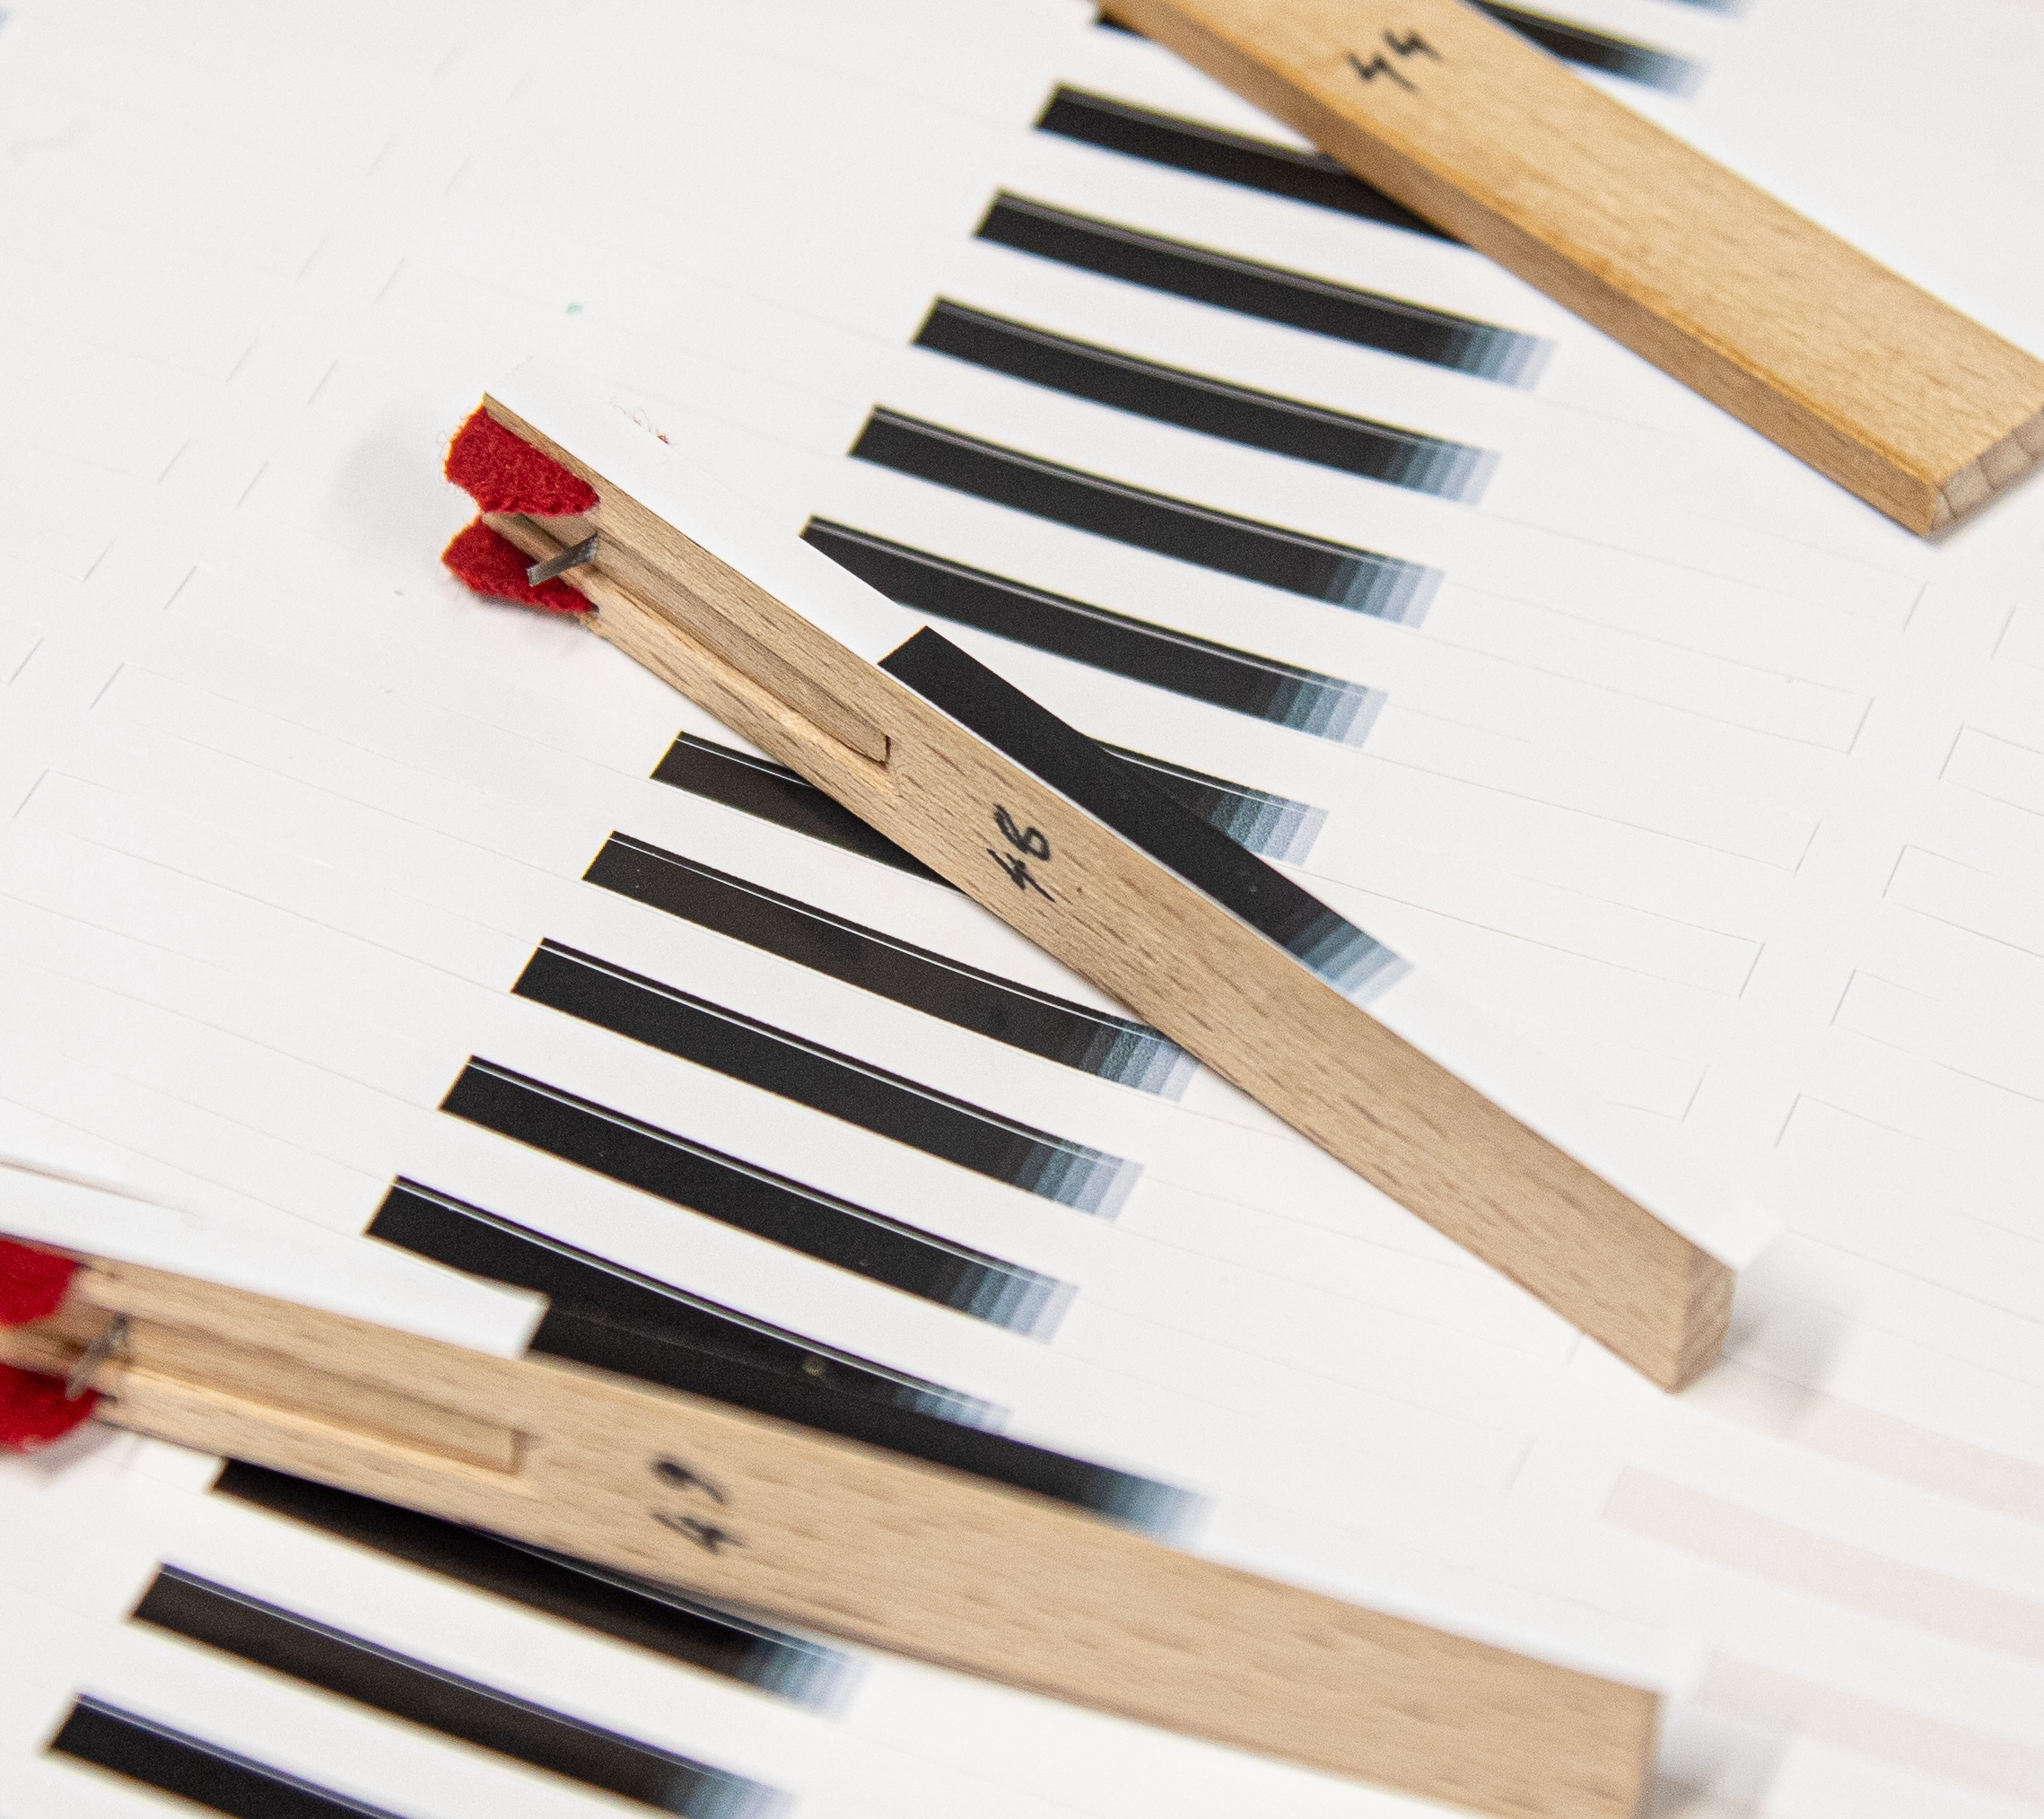
\includegraphics[width=0.9\linewidth,trim={0 0 0 0.5cm},clip]{src/images/tagging-jacks-3.jpg} 
  \caption{Gradient stickers applied to the side of the jack body. The coarse gradient scale was selected to maximise signal excursion while preserving signal readout stability.}
  \Description{} 
  \label{fig:jack-tags}
\end{figure}

Optical sensors are positioned in front of each jack and their output voltage depends on the amount of light reflected from a sensor surface. In this case, the sensor surface is a grey-scale gradient printed on a vinyl sticker (Figure \ref{fig:jack-tags}) and applied to the side of each jack. Though the current configuration simply sends MIDI note-on and -off messages when passing a threshold, the displacement of all jacks is available continuously.
The jacks for a single key typically have their pluck points offset from each other, a practice known as `staggering'.
A combination of string tension, quill voicing, and jack staggering contribute to the overall resistance of the action, with each key differing from the low to the high octaves \cite{Veroli2012}. The staggering of the pluck point of the jacks between registers means that there are two distinct tactile anchors along the key dip. The current sensor system enables the data recording of traditional use from which it can be identified where those opportunities for new expression lie \cite{McPherson2013-2}.

% "When working with an established interface like the keyboard, it is particularly important that new mappings do not interfere with familiar technique (McPherson, Gierakowski, and Stark 2013). The Space Between the Notes: Adding Expressive Pitch Control to the Piano Keyboard"

\begin{figure}
  \centering
  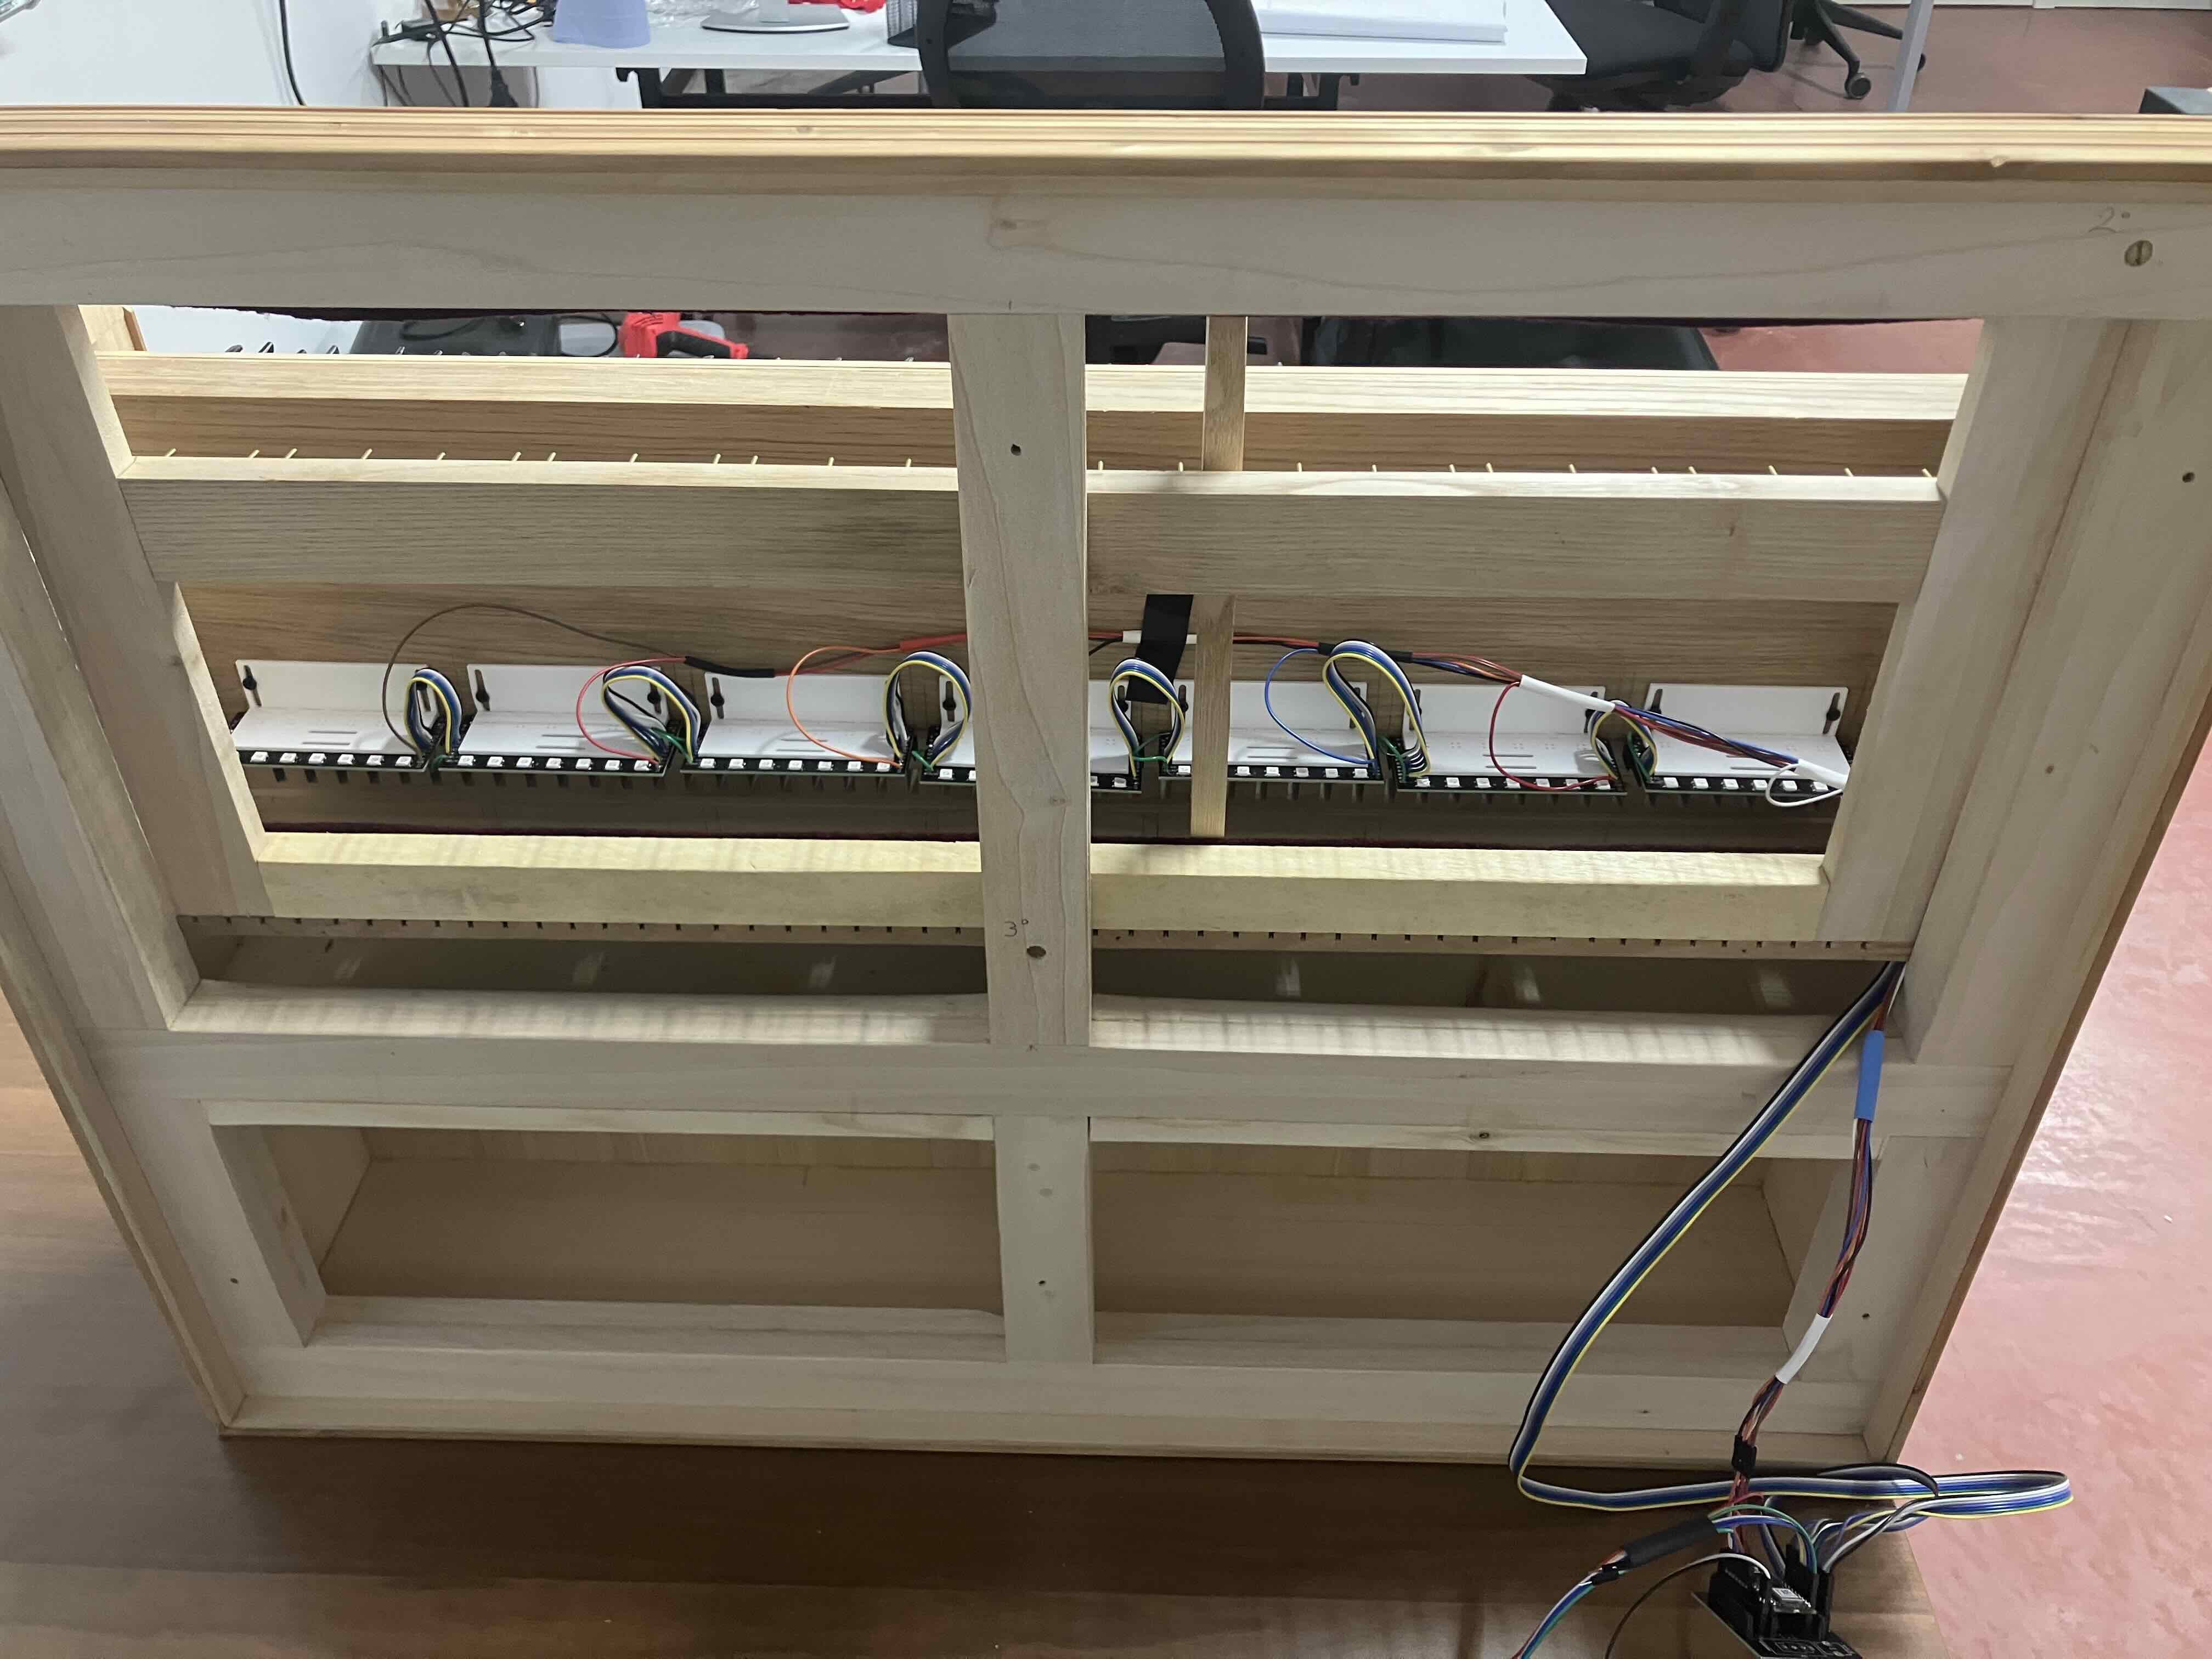
\includegraphics[width=\linewidth]{src/images/49-key-bottom-sensors-no-keys.jpg} 
  \caption{Underside of the full model keyboard, showing two chambers: the front chamber (top) and the rear chamber (bottom).} 
  \Description{} 
  \label{fig:49-key-bottom}
\end{figure}

A modular system of printed circuit boards (PCBs) was designed to manage the sensors and process their output. The system uses 49 optical sensors which are distributed across seven boards that contain 7 sensors each. The PCBs were secured to the underside of wrest plank and above the keys (Figure \ref{fig:49-key-bottom}), allowing them to be adjusted during installation. Ribbon cables connected the PCBs, providing flexibility during assembly while maintaining a compact form factor. Additional modifications, including baffles and adhesive improvements, were made to optimise the reliability of the sensor system during calibration and use.

The project expanded upon earlier NIME research on generating MIDI messages from piano keystrokes \cite{McPherson2013}, adapting it to address the specific characteristics of harpsichords. Whereas the previous design emphasised continuous gesture tracking, this implementation required discrete key-triggered data to align with the needs of MIDI-triggered audio playback. 

\subsection{Materials and Construction}
The keyboard was designed to replicate the tactile and aesthetic sensations of playing an historical Italian harpsichord. Traditional materials were used, including walnut for the wrest plank, chestnut for the key levers, boxwood and ebony for key covers, and cypress for the case and soundboard. The 98 jacks were made from beech, fitted with brass springs and natural seagull feather plectra. The design was inspired by Venetian harpsichords, particularly the \anon{1547 Alessandro Trasuntino} harpsichord at the \anon{San Colombano Museum}. An exception was made for the short octave --- the assigning of common keys in the first octave instead of a chromatic scale --- typically found in Italian harpsichords, which was replaced by a standard octave layout to more easily accommodate the interaction with commercial sample libraries. 

% % Option 2
\begin{figure}[!b]
    \centering
     \begin{subfigure}[h]{0.4\linewidth}
        \centering
        \includesvg[inkscapelatex=false, width = \linewidth]{images/log_harp_outline}            
        \caption{logarithmic shape}    
        \label{fig:log-harp}
    \end{subfigure}

    
    \begin{subfigure}[h]{0.4\linewidth}
        \centering
        \includesvg[inkscapelatex=false, width = \linewidth]{images/49-key_outline}        
        \caption{rectangular shape}
        \label{fig:rect-harp}
    \end{subfigure}
    \caption{Logarithmic shape of an original \anon{Trasuntino} harpsichord contrast with the rectangular shape of the replica}    
    \Description{}
    \label{fig:log-harp-comp}
\end{figure}

The rectangular poplar frame also deviates from the traditional logarithmic (Figure \ref{fig:log-harp-comp}) form to allow for the installation of the electronic sensors, as visible in Figure \ref{fig:49-key-bottom}, without compromising the visual or tactile authenticity. Two string choirs, crafted from yellow brass wire and anchored with wrought iron pins, were tensioned to replicate authentic plucking resistance. Felt strips were added to dampen vibrations. The result is an interface that combines the mechanical action of keys with synthetic sound generation, preserving a real harpsichord's tactile qualities.


\subsection{Project Deployment}

A further objective, set forth by the authors, was to ensure reproducibility by committing to an open source approach for all outputs of the project. The commitment to open sourcing encompassed all aspects of the system, including hardware schematics, firmware, and calibration data. Cost-effectiveness was also a central consideration. 
% The system was initially developed for a 3-key prototype, shown in Figure \ref{fig:3key}, and successfully scaled to 49 keys without significant increases in cost or complexity. 
Specifically, the system was designed to be easily assembled using resources typically available in a university-managed maker space. Components, such as QRE1113 optical sensors and CD4051BE multiplexers, are widely available from commercial resellers, while the modular PCB design ensures easy replication and maintenance. The Arduino Nano was chosen as the core microcontroller format for its compatibility with open source tools. Calibration workflows were optimised using the Arduino IDE’s serial plotter and open source MIDI Monitor software \footnote{\url{https://github.com/krevis/MIDIApps}}, reducing reliance on proprietary tools and simplifying the process for users. 

\begin{anonsuppress}
Reference repositories for this project can be found here:

    \begin{itemize}
        \item 
        \emph{Firmware}: \anon{\url{https://github.com/Nemus-Project/harpsichord-interface-firmware}}
        \item 
        \emph{PCB CAD}: \anon{\url{https://github.com/Nemus-Project/harpsichord-interface-cad}}
        \item 
        \emph{Interface Models}: \anon{\url{https://github.com/Nemus-Project/harpsichord-interface-models}}
    \end{itemize}
\end{anonsuppress}


\section{Hardware Design}\label{hardware-design}

\begin{figure*}
    \centering
    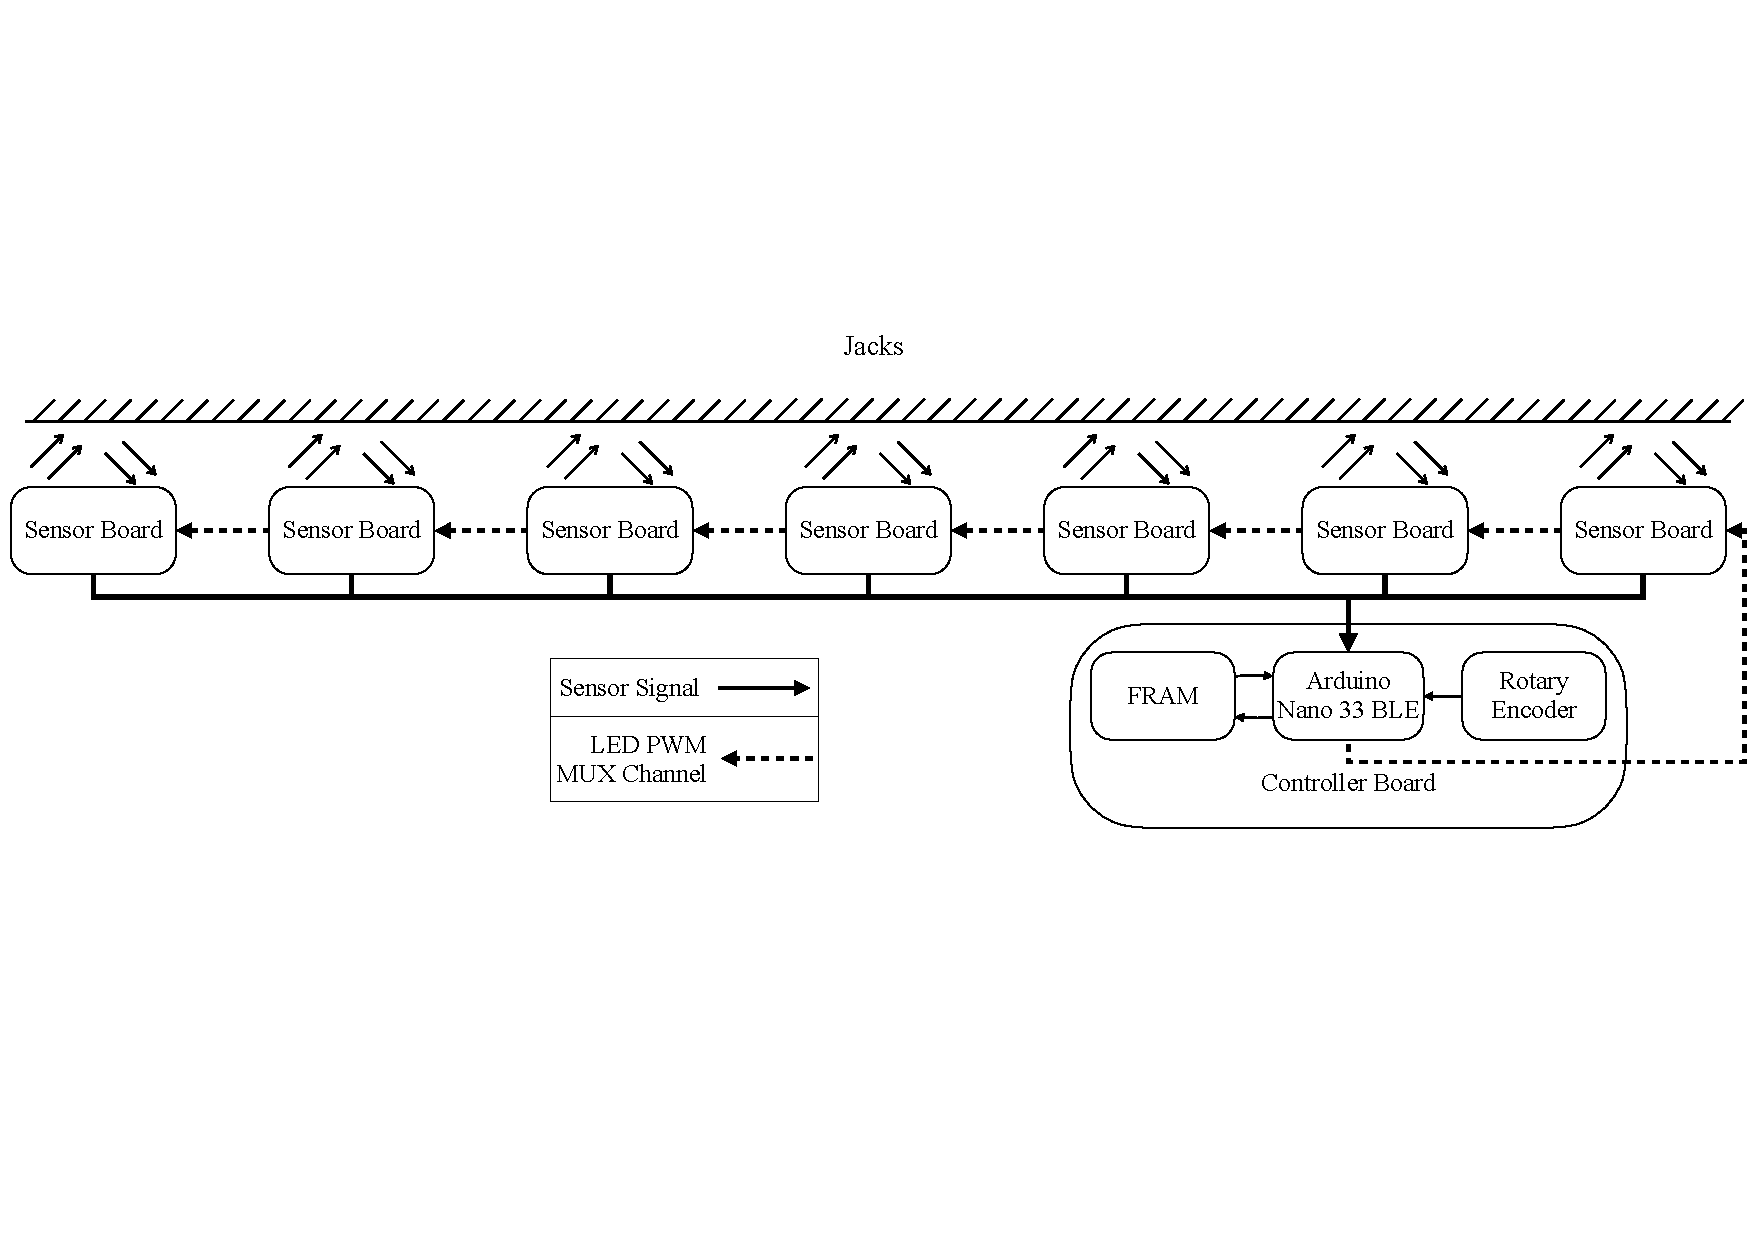
\includegraphics[width=\linewidth]{src/images/block-diagram-2.pdf}
    \caption{Block diagram of PCB connections. A separate sensor signal is routed to the Arduino. LED and multiplexer (MUX) controls signal are daisy-chained through each sensor PCB.}
    \label{fig:system-block-diagram}
\end{figure*}

Figure \ref{fig:system-block-diagram} shows a block diagram of the finalised hardware setup. 
The system evolved through iterative prototyping, beginning with simple threshold-based testing and ending in a fully functional multi-sensor interface capable of triggering MIDI events. 

\begin{figure}
    \centering    
    \includegraphics[width=\linewidth]{src/images/3-key-side.png}
    \caption{
    3-Key Model Harpsichord Mechanism    
    %acquired from \anon{San Colombano, Bologna}, 2023.
    }
    \label{fig:3key}
\end{figure}

\subsection{Prototype Stage}

The initial stage of development focused on testing whether sensor data could reliably trigger MIDI playback. Modifying an existing harpsichord for testing was considered but ultimately discarded due to significant internal measurement and layout discrepancies. Instead, a custom 3-key harpsichord mechanism (Figure \ref{fig:3key}) was used as a foundation for prototyping. This approach followed a methodology similar to that used in Timmermans \emph{et al.}'s Haptic Key project \cite{Timmermans2020}, since the 3-key model enabled iterative testing of individual components, including sensor placement, signal processing, and mechanical tolerances, before upscaling. 

The following criteria were established to guide sensor selection and integration to make the system suitable for a museum context:

\begin{itemize}
    \item \emph{Non-invasiveness:} No remarkable modifications were allowed on the harpsichord mechanics, particularly on all the visible parts.
    \item \emph{Low Latency:} The sampling period for reading and processing data from all sensors should remain under 10 ms to allow for latency introduced in other parts of the synthesis process. Empirical criteria found in previous studies \cite{Jack2016} was used as a guide.
    \item \emph{Reliability:} Sensor data should be dependable and consistent, with interference from anything external to the jack movement being absent or negligible.
    \item \emph{Scalability:} The design needed to scale in both cost and time in order to be adaptable from a 3-key prototype (Figure \ref{fig:3key}) up to the 49 keys of the final design.
    % \item \emph{Expandability:} The system should accommodate future functionality, such as additional MIDI parameters or data visualisation.
\end{itemize}

The hardware was designed to make assembly possible in standard university maker spaces.  

\subsection{Sensor Board}\label{sensor-board}

\begin{figure}[!h] 
  \centering
  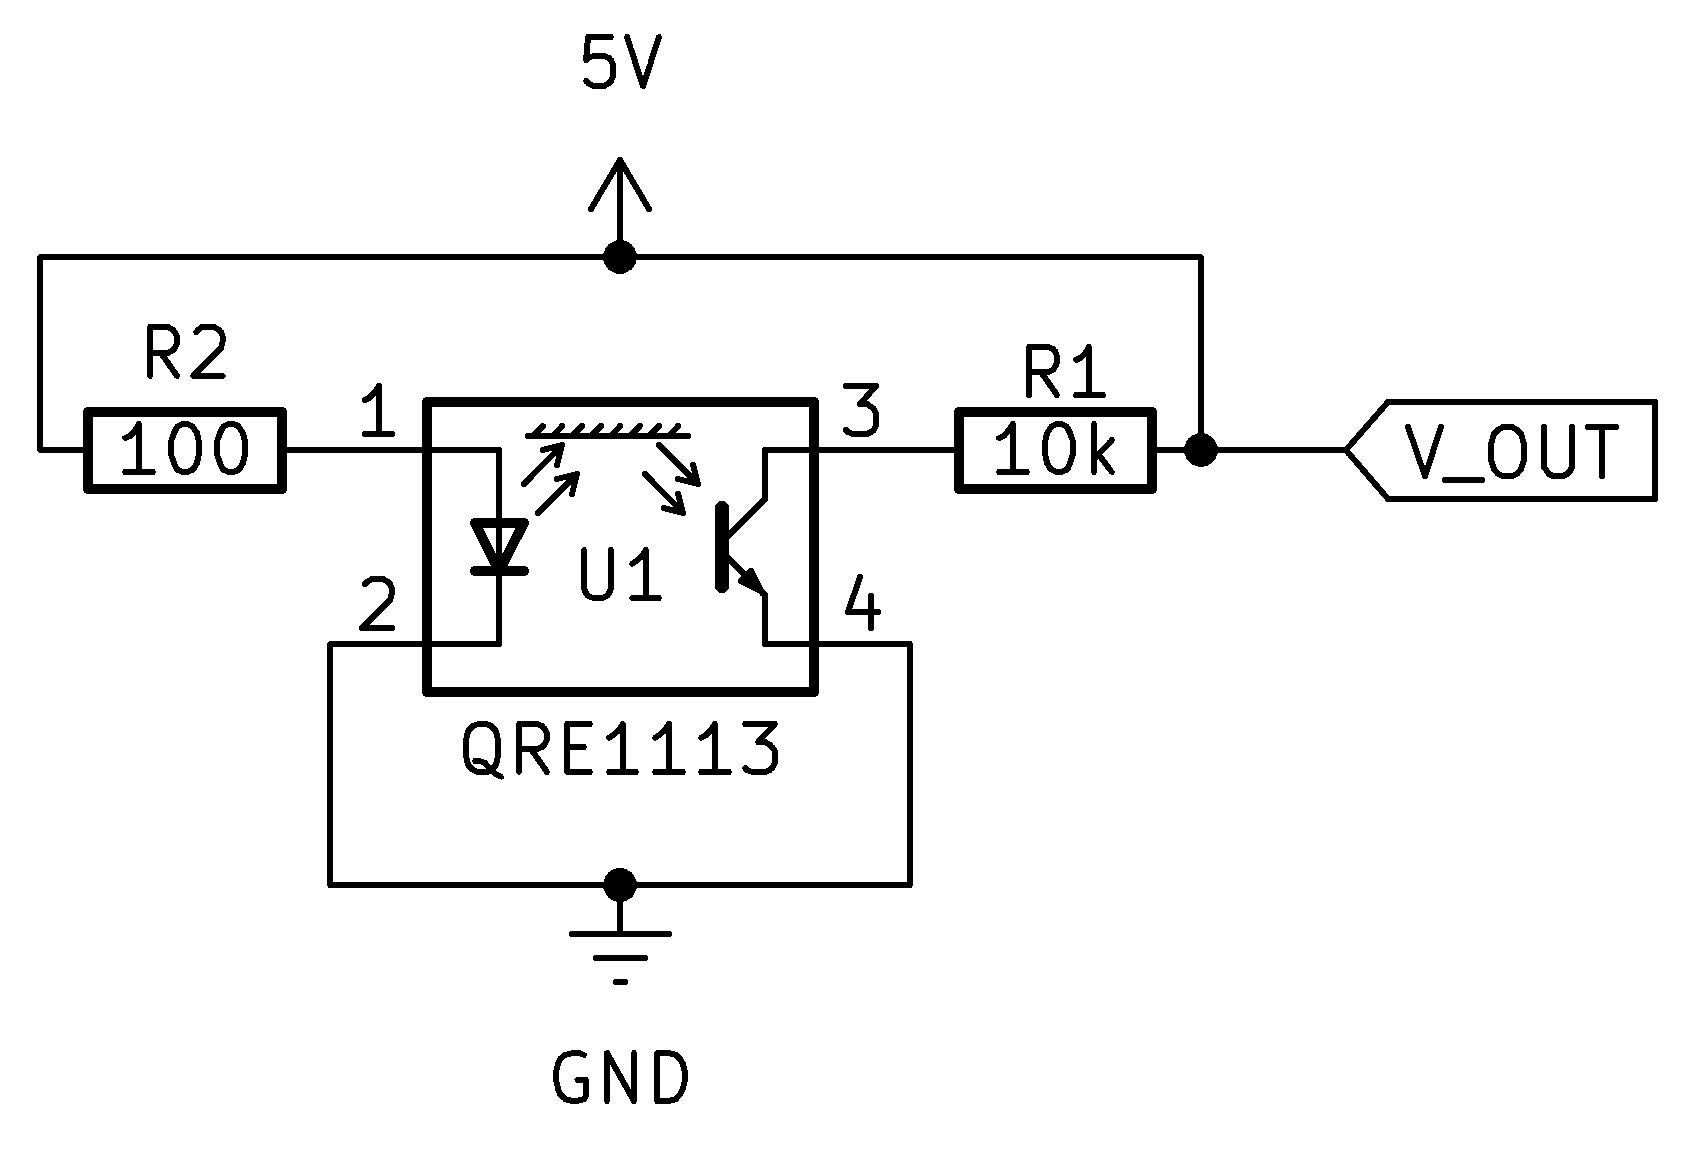
\includegraphics[width=0.7\linewidth,trim={0 0.5cm 0 0.5cm},clip]{src/images/simple-schematic-bw-.jpg} 
  \caption{Optical sensor in a simple voltage divider circuit. \texttt{V\_OUT} is routed to one of 8 channels on the CD4051BE multiplexer.}
  \Description{} 
  \label{fig:simple-schematic}
\end{figure}

The final sensor system utilised QRE1113 optical sensors, known for their small form factor, low cost, and suitability for short-range distance detection \cite{McPherson2013, McPherson2019}. The sensors were distributed across seven printed circuit boards, each responsible for seven keys. Each PCB contained the following components:

\begin{itemize}
    \item 7 QRE1113 optical sensors.
    \item 7 100 $\Omega$ resistors and 7 10 k$\Omega$ resistors (later reduced to one resistor per board).
    \item 1 Texas Instruments CD4051BE multiplexer for signal aggregation.
    \item 7 WS2812 RGB LEDs with integrated driver.
\end{itemize}

The optical sensors are wired in a voltage divider configuration (Figure \ref{fig:simple-schematic}) and the circuit outputs a voltage based on the infrared light reflected from nearby surfaces. 
The gradient stickers affixed to each jack provided a surface with varying reflectivity for the sensors, which were used to track jack displacement throughout the key dip. 

\begin{figure}[!t]
    \centering
    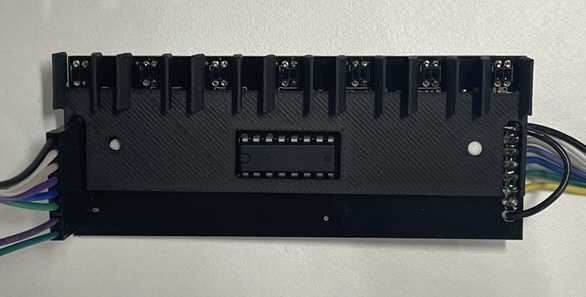
\includegraphics[width=\linewidth,trim={0 1.5cm 0 1.5cm},clip]{src/images/sensor-board-w-baffles.jpeg}
    \\
    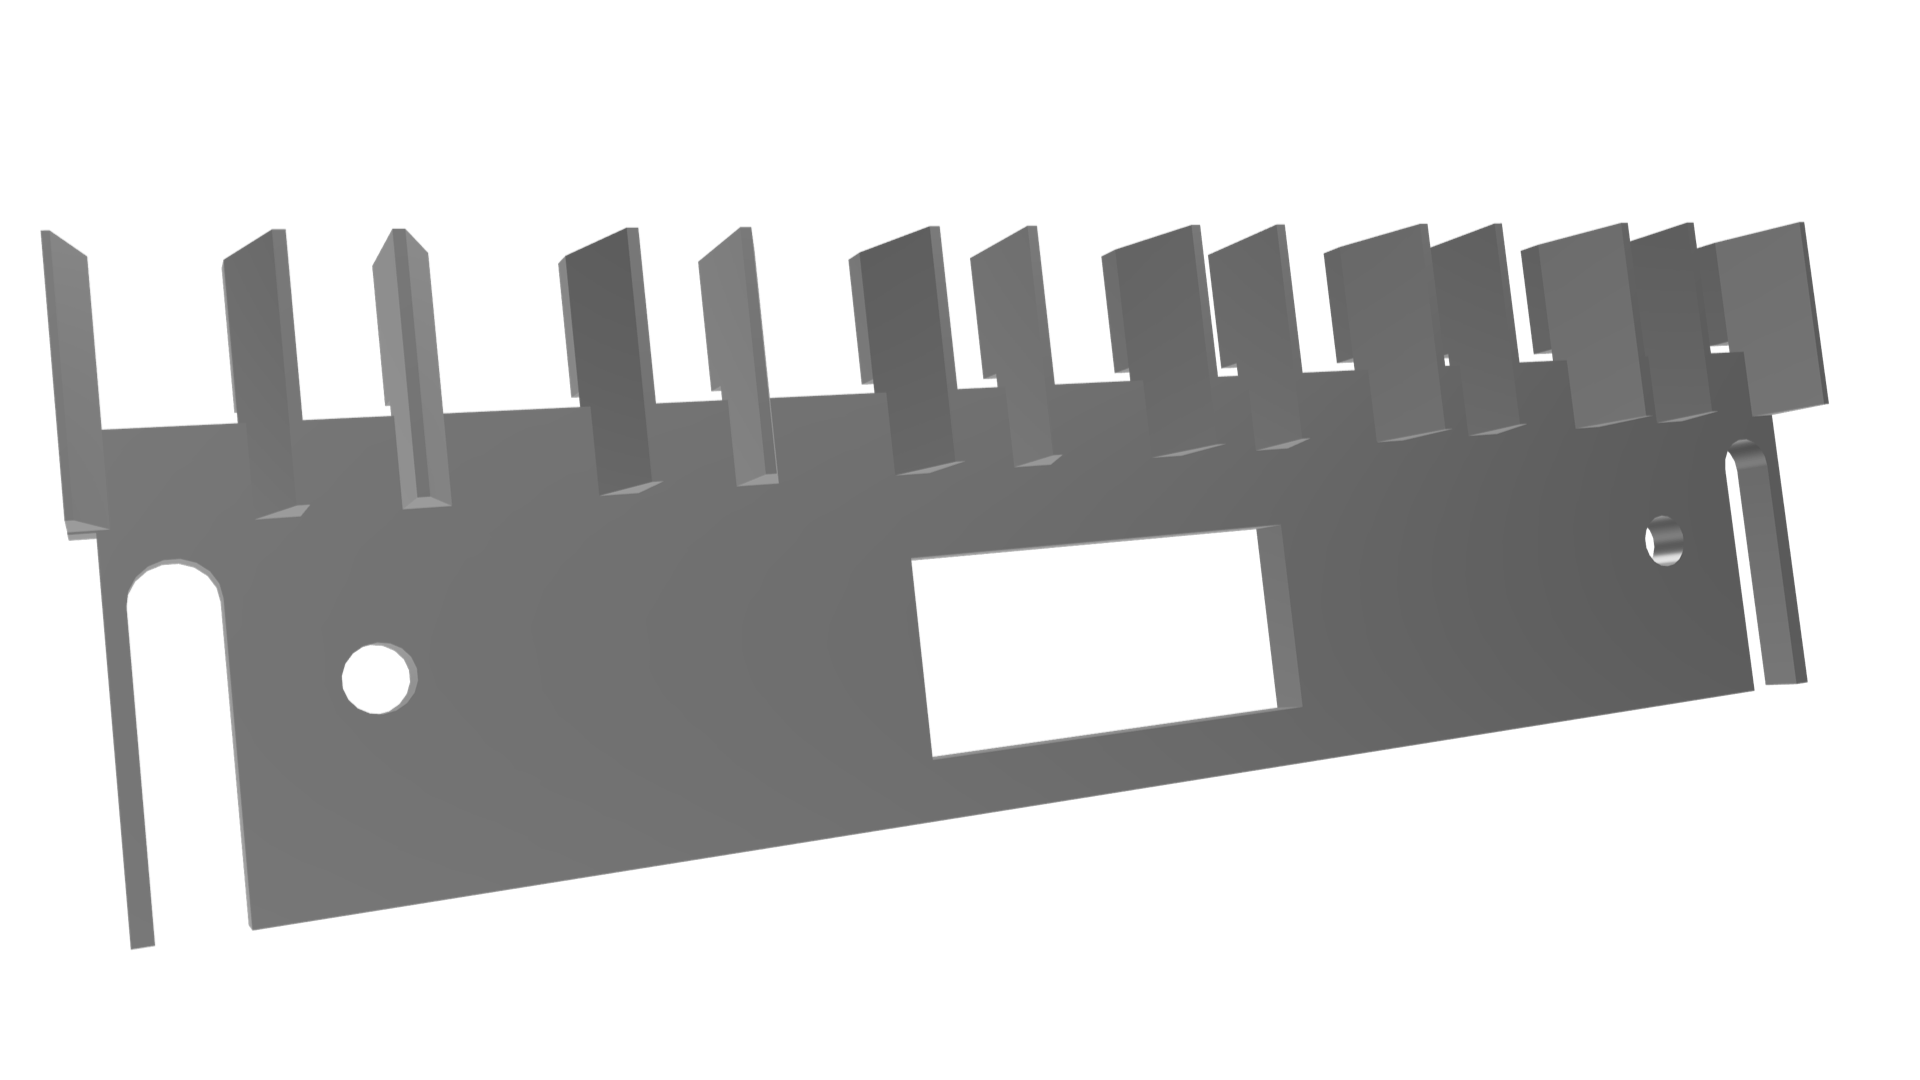
\includegraphics[width=0.8\linewidth,trim={0 2cm 0 2.5cm},clip]{src/images/baffles.png}
    \caption{Baffles designed to prevent cross-talk between adjacent sensors.}
    \Description{}
    \label{fig:baffles}
\end{figure}

3D-printed baffles were installed on the PCBs to eliminate cross-talk between adjacent sensors, as per Figure \ref{fig:baffles}. These baffles, fabricated from dark-pigmented PLA, ensured that infrared reflections from neighbouring jacks did not interfere with sensor readings. A manual visual check of plotted all sensors readings confirmed that interference from neighbouring jacks had been eliminated. RGB LEDs are placed on the reverse side of the PCB, vertically in-line with the sensors, and were added to provide a programmable means of providing visual feedback. The LEDs are controlled via a pulse width modulation (PWM) signal and are addressable individually.
The output signal of the multiplexer is taken from each PCB and routed to a separate ADC channel of the Arduino. Multiplexer channel select and LED PWM signals are daisy-chained through each PCB (Figure \ref{fig:sensor-reverse}).

\begin{figure}[!b] 
  \centering
  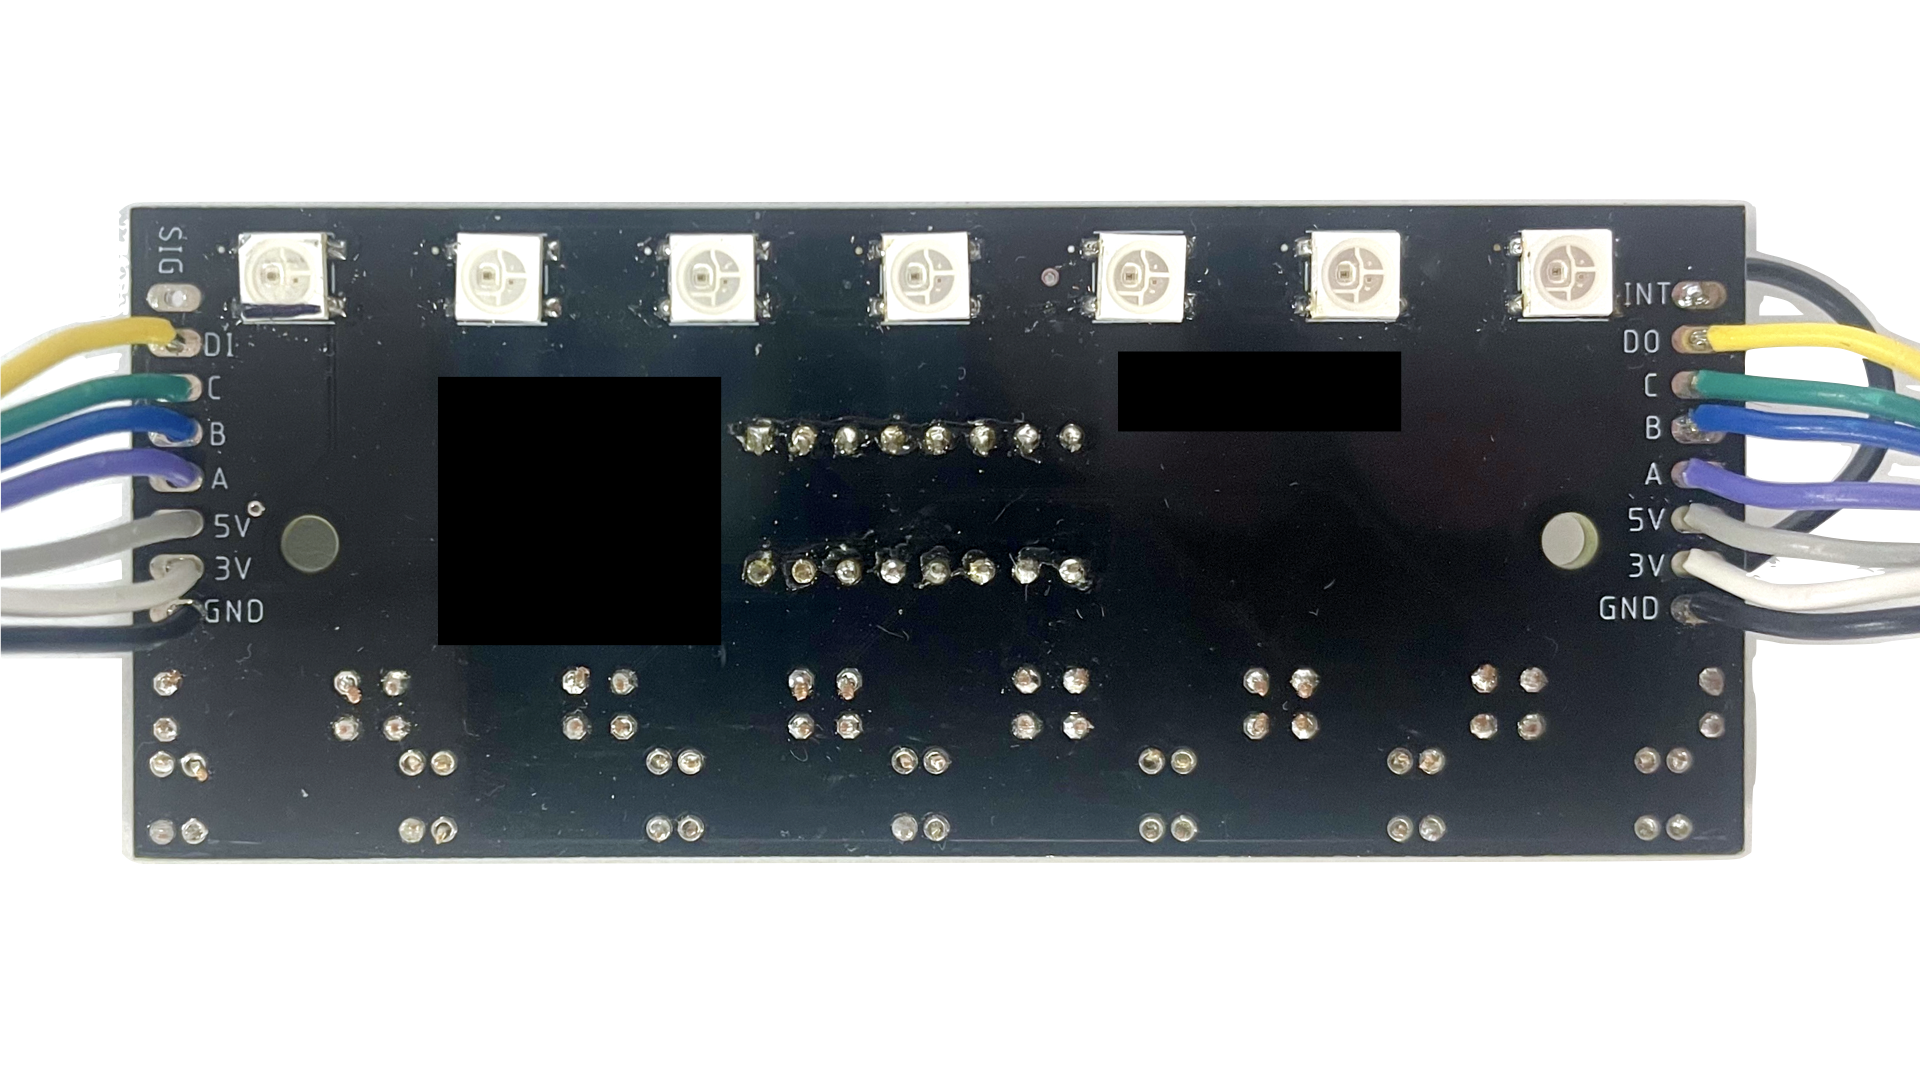
\includegraphics[width=\linewidth]{src/images/sensor-board-reverse-side-anon.png} 
  \caption{Reverse side of the sensor board showing the RGB LEDs and terminal connections. The \texttt{SIG} terminal (Top Left) is routed to an ADC channel. Power \texttt{5V, 3V, GND}, multiplexer channels \texttt{A, B, C} and LED PWM input \texttt{DI} and output \texttt{DO}  connect from the previous sensor board (Left) and are routed to the next (Right).}
  \Description{} 
  \label{fig:sensor-reverse}
\end{figure}

\subsection{Controller Board}\label{controller-board}

The controller board, designed around the Arduino Nano format, was the central hub for processing sensor data and triggering MIDI messages. In addition to solder terminals for the sensor board channels, the controller board contained:

\begin{figure}[!t]
    \centering
    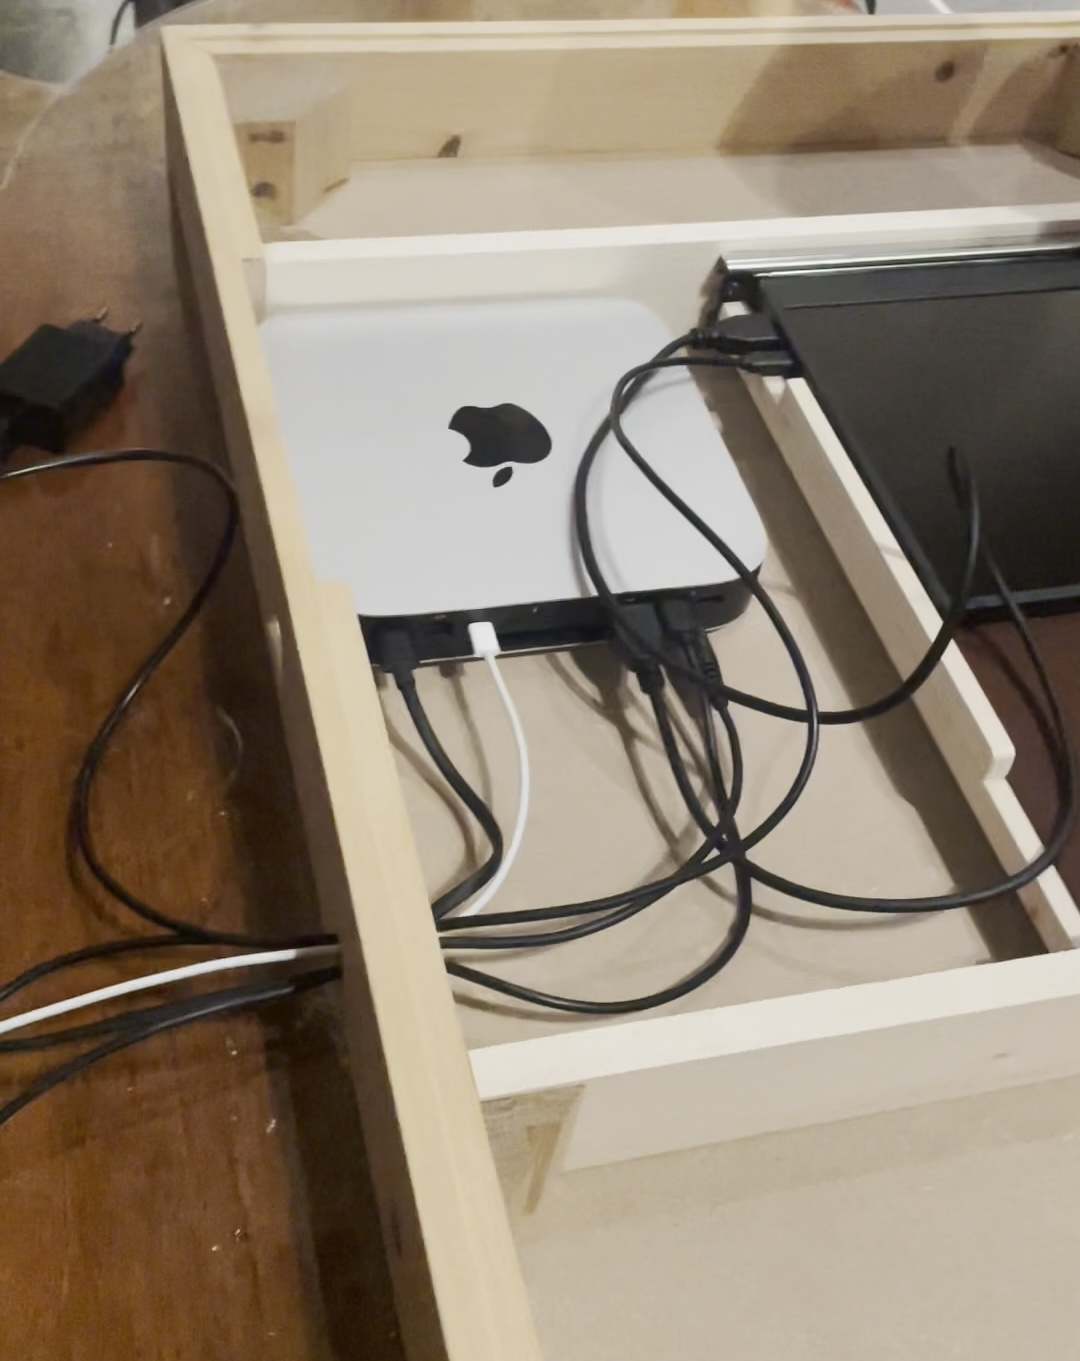
\includegraphics[width=0.8\linewidth,trim={0 5cm 0 0},clip]{src/images/mac-mini.jpg}
    \caption{Components and cabling hidden in the bottom section of the instrument case.}
    \label{fig:mac-mini}
\end{figure}

\begin{itemize}
    \item 1 Arduino Nano 33 BLE.
    \item 1 Fujitsu MB85RS64 SPI Ferroelectric RAM chip.
    \item 1 EC11 combined rotary encoder and tactile switch.
    % \item 1 DFROBOT DFR0785 Tactile Switch
\end{itemize}


The Arduino Nano's small form factor made fitting the board inside the harpsichord easier and also allowed for testing of multiple chipsets. The 33 BLE variation of the Nano had the additional benefit in its ability to be programmed as both native USB MIDI and BLE MIDI devices. The 33 BLE was also able to achieve a sampling period of 1.7 milliseconds for all sensors. A 4-sample moving average filter was implemented to reduce noise and brought the effective sampling period to 5.1 milliseconds.
% Samping period was measure by timing each iterations of the entire sensor read and processing cycle, polling the internal clock of the arduino a the start and end of each cycle and storing the difference in a buffer.  After 10k cylces the buffer of timing was sent over serial and a mean average of 1.7 milliseconds was found with a jitter of ±0.2 milliseconds.

Non-volatile memory, implemented using a Fujitsu MB85RS64 Ferroelectric RAM (FRAM) chip, provided a reliable means of storing and preserving calibration settings across power cycles. This ensured that sensor thresholds and other settings could be preserved across power cycles, enhancing the system's usability in museums.  

A rotary encoder was used as the interface to select a key, edit a threshold and save current thresholds to the FRAM.
Thresholds were first set the midrange of possible values a a default. A rough calibration process was carried out where each sensor were selected individually and its readings were plotted against their current threshold value using the Arduino IDE serial plotter. Thresholds were adjusted with the rotary encoder until the key no longer passed the threshold line until the jack had plucked the string. During calibration RGB LEDs were used as a visual aid to quickly identify which key was currently being adjusted. These LEDs also provided visual feedback during calibration, and would change colour based on if readings were above below the threshold or if the were outside previously recorded maximum or minimum values. Such use of the LEDs meant for easy identification of malfunctioning sensors and simplified the alignment process. A finer calibration process was carried out with the guidance of expert harpsichord performer \anon{Catalina Vicens}.

Power requirements for the system were estimated at 1.1 A at 5 V, with some fluctuation when the system was first powered on. While the sensors were powered continuously in this iteration, future designs may incorporate power-saving measures, such as dynamic modulation of the optical emitters found in the McPherson piano \cite{McPherson2013}.

For the initial version of the exhibition, a harpsichord sample library was used and controlled via Native Instrument's Kontakt\footnote{\href{https://www.native-instruments.com/en/products/komplete/samplers/kontakt-8/?srsltid=AfmBOorKUf43SoIxGBS2-GnXmKHHkgcfcfWRskpweDhLSG3FiF0qrf2w}{Kontakt webpage} (accessed 31 Jan 2025)}. The software was installed on a Mac Mini hosted inside the instrument's case. Holes were drilled at the back of the instrument's frame, away from sight, to allow the passage of cables, such as from power supplies, USB connectors and headphone jack (Figure \ref{fig:mac-mini}). 
An iPad is used as a monitor through which visitors can adjust playback parameters such as tuning, voicing and which stops are engaged. The next iteration will use a library of samples from instruments in the collection, which the museum is currently carrying out.



\section{Discussion}\label{context}

% In an effort to make the exhibition more accessible and authentic, the \anon{San Colombano Museum} commissioned the construction of a mechanical keyboard to trigger a MIDI-controlled sample library, designed for use by museum visitors. 
The exhibition is set to open approximately a month after this work's submission, and only preliminary feedback has been collected from a pool of 20 people -- consisting of staff, surveillance personnel and visitors who were given training on the system -- and expert feedback from \anon{Catalina Vicens} and \anon{Roberto Livi}.
The collection of visitor feedback was carried out as short informal interviews and primarily as a means of identifying any technical problems.
The keyboard shows promise in enhancing the museum experience as comments about a ``sense of disconnect'' found in the Benton Fletcher Collection \cite{McAlpine2014} were absent in this initial feedback.

%\textcolor{red}{This goes in the direction pointed by Andrew, but I wonder if it could be worded differently}

A more formal surveying of museum visitors is to be carried out to determine to what degree the exhibition achieved its core aims.
The keyboard is hosted in the \emph{Oratory} above the museum's main hall, an exceptional testimony to the Bolognese art, decorated by the finest students of the Carracci and presenting a series of frescoes covering most of the walls and ceiling. The room hosts unique examples of the Italian Renaissance building tradition, including the 1547 harpsichord and the 1540 spinet by \anon{Alessandro Trasuntino}. Visitors often visit the room with the same caution and respect typical of worship spaces. Among the visitors interviewed, no comments were made that the exposed headphones and touchscreen affected such an experience negatively, though a more definitive answer will come as more feedback is collected after launch. Pictures of the keyboard hosted in the \emph{Oratory} are shown in Figure \ref{fig:oratory}.

Expert feedback has highlighted limitations, including imprecise key calibration, which creates a temporal disconnect between the tactile plucking sensation and sound onset. Additionally, the commercial sample library, while allowing the selection of registers such as 8', 4', and their combinations, restricts functionality to a single MIDI message per key, regardless of the number of string choirs controlled. Inspired by early Italian instruments, the keyboard's layout is designed to manage two 8' registers with a sensor system fitted to each. Internally, the instrument functions as two separate MIDI devices. However, one register must be disengaged due to the software's limited communication with only a single device. While running multiple instances of the software is possible, having two sets of GUI controls was considered too confusing for visitors engaging with the exhibition without prior orientation. Consequently, sensors are only active on single jacks to accommodate these constraints. Future iterations could address these limitations through technical improvements, such as refined calibration with hysteresis and developing a custom sample library and interface.


\begin{figure}
\centering
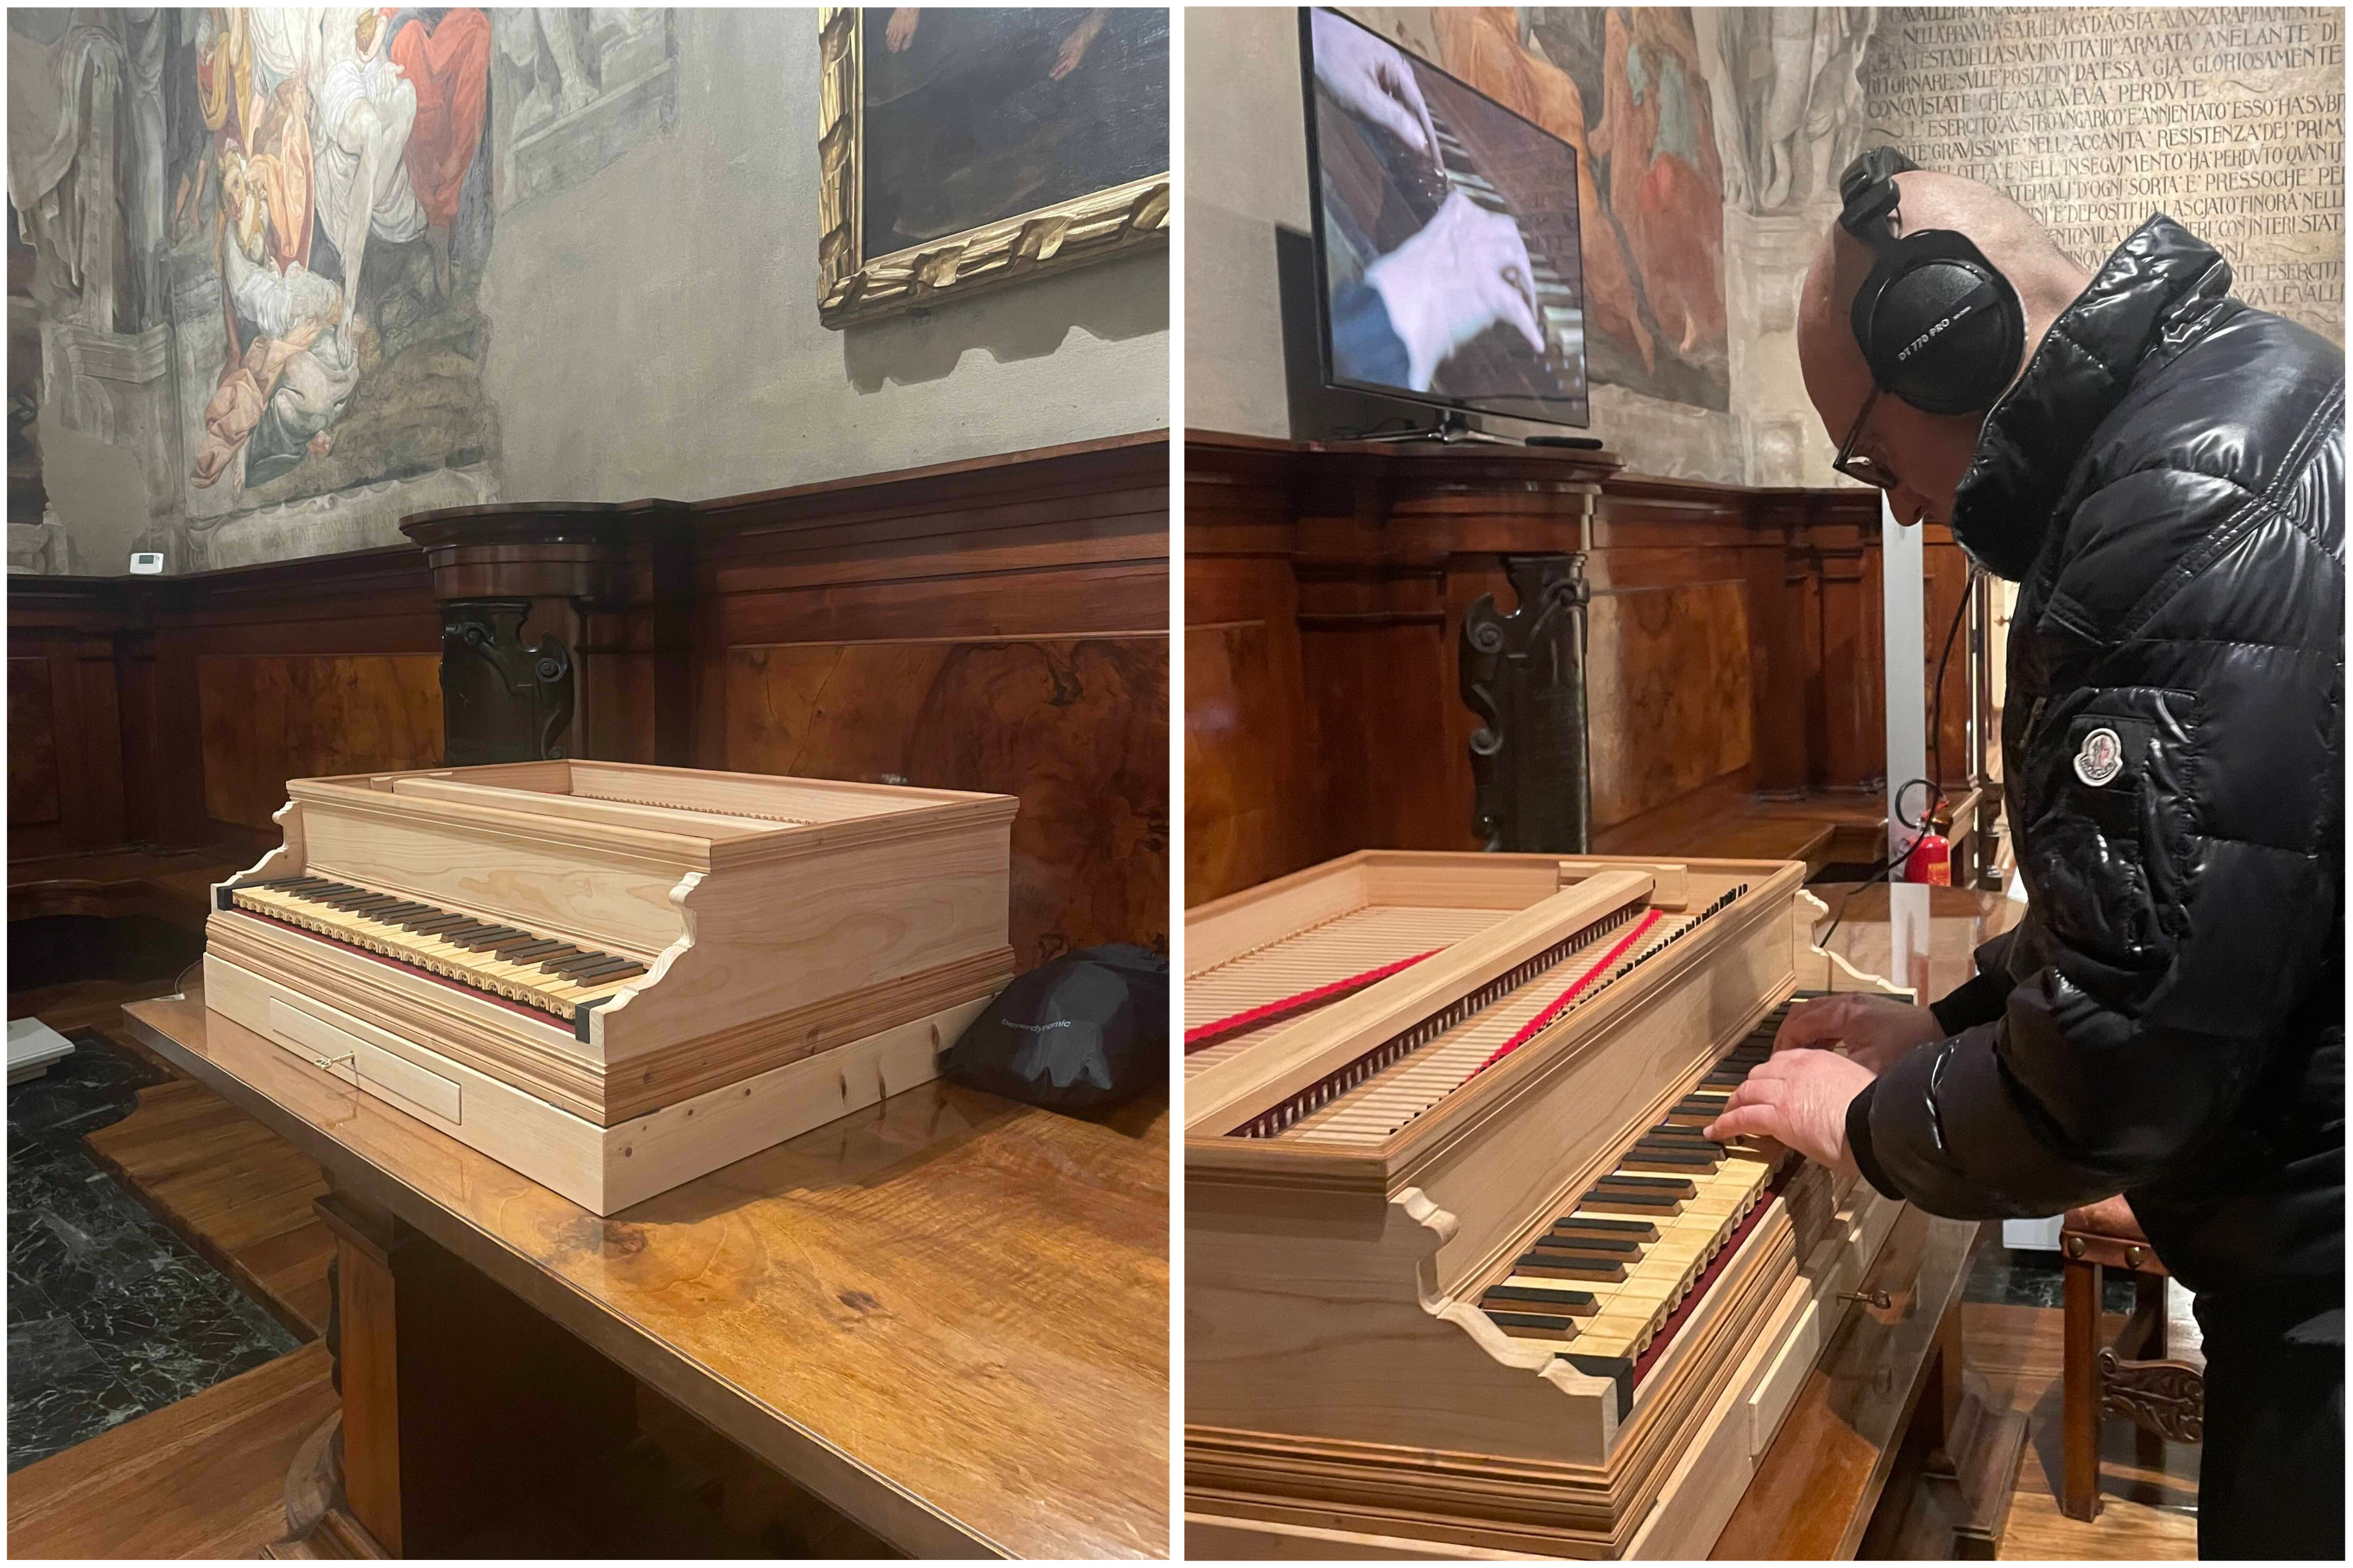
\includegraphics[width = \linewidth]{src/images/keyboardMuseum.JPEG}
\caption{The keyboard installed in the \emph{Oratory} at \anon{San Colombano}, and a user wearing headphones playing it.}
\label{fig:oratory}
\end{figure}

A longer discussion, but one going beyond the scope of this work, is whether the current setup or its future iterations may be effectively used to build legitimate replicas of historical musical instruments or even become a kind of \emph{new} musical instrument altogether. As such, the question is whether these designs may result in music being practised, performed and recorded with the instruments. This work supports an overarching narrative extending beyond its application in museum collections. The \anon{NEMUS project \cite{NEMUS}}, focusing on developing advanced physical models simulating the non-linear interaction between subcomponents, has commissioned a second keyboard to further explore the role of control interfaces in performance, employing the sense of touch as link between the mechanical world with the digital, replicating the embodied relationships between performer and instrument and offering opportunities to modify or even disrupt these interactions. The upcoming Rem@ke project \cite{remake1} has also expressed an interest in engaging with the keyboard to explore meaningful embodied interactions between players and instruments. 

% \section{Conclusion}\label{conclusion}

% This study has presented the design and implementation of an electronically augmented keyboard for the Tagliavini Collection at the San Colombano Museum. By leveraging optical sensors and MIDI-controlled sample libraries, the keyboard allows users to explore a harpsichord's sonic and mechanical essence without compromising the integrity of the museum's historical artefacts. Preliminary feedback shows that the keyboard has the potential to enhance the museum experience, particularly for those unfamiliar with early keyboard instruments. However, technical limitations, such as calibration inconsistencies and restrictions imposed by the commercial sample library, highlight opportunities for refinement. These issues will be addressed in future iterations, including a second keyboard designed to control advanced physical models. This work opens new possibilities for engaging with heritage collections while respecting their authenticity. It also serves as a foundation for further research projects exploring embodied cognition in historical instruments, and it may provide a useful framework to investigate the links between physical modelling and digital musical interface design.

